% This is LLNCS.DEM the demonstration file of
% the LaTeX macro package from Springer-Verlag
% for Lecture Notes in Computer Science,
% version 2.3 for LaTeX2e
%
%\documentclass{llncs}
\documentclass{IEEEtran}
%
\usepackage{makeidx}  % allows for indexgeneration
\usepackage{algorithmic}
\usepackage{algorithm}
\usepackage{xspace}
\usepackage{array}
\usepackage{eqparbox}
\usepackage{forest}
\usepackage{caption}
\usepackage{graphicx}
\usepackage{subfigure}
\usepackage{pgfplots}
\usepackage{color}

\newcommand{\bug}
    {\mbox{\rule{2mm}{2mm}}}
\newcommand{\Bug}[1]
    {\bug \footnote{BUG: {#1}}}
\newcommand{\pf}{predictive forest\xspace}
\newcommand{\PF}{Predictive Forest\xspace}
\newcommand{\pt}{predictive tree\xspace}
\newcommand{\PT}{Predictive Tree\xspace}
\newcommand{\TPR}{Time-Parametrized R-Tree}
\newcommand{\tpr}{time-parametrized r-tree}
%\renewcommand\algorithmiccomment[1]{%
%  \hfill//\ \eqparbox{COMMENT}{#1}%
%}

%
\begin{document}
%
%\frontmatter          % for the preliminaries
%
%\pagestyle{headings}  % switches on printing of running heads
%\addtocmark{Hamiltonian Mechanics} % additional mark in the TOC
%

\title{Predictive Forest: An Incredible Data Structure for Querying Moving Objects under Uncertainty}

\author{
{Abdeltawab M. Hendawi, Abdelrahman Elogeel, Rahul Deshpande, Mohamed Ali}
\institute{Department of Computer Science and Engineering, University of Washington, Tacoma, WA 98402, USA}
\email{hendawi@uw.edu, elogeel@uw.edu, deshpr@uw.edu, mhali@uw.edu}
}

\maketitle

\begin{abstract}
The current pose of the mobile devices help in reporting locations on their holders to open a brand new research opportunities. Yet, the provided locations will not always be precious as the network coverage stability is not granted. To answer a moving object predictive query, algorithms assuming uncertainty will probably hold relevant results more than certain ones. In this paper, we present \pf, a data structure for querying moving objects under uncertainty. We accuracy and scalability experiments over moving objects in Washington state and compare results with \tpr.
\end{abstract}

\chapter{INTRODUCTION}
\label{sect:introduction}
% - motivation and example: uncertainty in location and time.
The availability of mobile devices with Global Positioning System (GPS) opened the gate for the research on moving objects. The GPS systems are able to tell what is the location of the moving object holding the mobile device. However, due to environmental and connection challenges, it is not guaranteed that the GPS sends an exact, accurate and certain location introducing location uncertainty challenges into play. Some scenarios require predictive queries, in which querying objects' future position is needed. In turn, this type of queries imposes an additional challenge, that is another dimension of uncertainty in time.

%These predictive queries impose uncertainty in time, for example a user could query for number of objects available in a specific location after some time.

% - quick survey on the existing work
The current literature is able to overcome the moving object uncertainty by following one of two different approaches:
\begin{itemize}
\item \textbf{Indexing} \cite{Zhang09} assuming that the object's past location and velocities are unknown $B^x-tree$ is utilized to provide techniques that can find anticipated objects' locations
in non-deterministic format.
\item \textbf{Modeling} assuming that the object moving pattern is uncertain, Recursive Motion Function (RMF) can model such patterns in different shapes like ellipse, circle, etc...
\end{itemize}

% - what we propose: how to use it, what are new features, how it works, describe internal operations, describe controlling parameters.
In this paper, we present a data structure called \pf used for querying moving objects and answering predictive queries under uncertainty. The benefit of using \pf is the ability to predict future steps for a moving object under time and location uncertainty. Given a road network (roads represent edges and intersections represent nodes), location uncertainty range (radius that describes the extent of location uncertainty), time range (integer value in seconds that describes for how long the \pf should predict) and probability threshold (to control the probability of nodes held in the \pf and ignore others below the threshold) the \pf provides prediction for the moving object steps. The \pf data structure offers two main operations $build$ to build an initial forest for the moving object without predicting any steps, and $update$ to predict what would be the next steps for the moving object along with probability assignment for each candidate node in the road network.

% - hint about experimental evaluation
The \pf prediction accuracy is compared with \tpr in the experiments which shows that \pf accuracy holds better than \tpr when the uncertainty increases by increasing the uncertain region radius.

% - describe rest of the paper
%In the rest of the paper, related work in the uncertainty literature is discussed then, \pf mechanics and algorithms are explained afterwards, we skim over the competitive algorithm \tpr and finally experiments and conclusion.

In the rest of the paper, we discuss related work in the uncertainty literature. Then, we explain the underlying mechanics and algorithms of the \pf data structure. Later on, we go over one of the competing algorithms (\tpr) highlighting some of its important aspects. Afterwards, we list experiments employing \pf and their results. Finally, we finish with our conclusions.

% - look at uncertainty paper Abdeltawab emailed and survey paper on his page

\input{"related\space work"}

\input{"predictive\space forest"}

\chapter{EVALUATION}
\label{sect:evaluation}
We conduct experiments on \pf using probability computation algorithm mentioned in Algorithm \ref{alg:prob} and compare results with \TPR.
\section{Experimental setup info}
The objects data are provided from real Washington state moving objects data. The section is divided into accuracy experiments, efficiency experiments and finally scalability experiments. The experiments were run on an Intel Core i7 2.4GHz CPU with 12GB RAM under Windows 8.1.
\section{Accuracy Evaluation}
\begin{itemize}
\item what is the chart about
\item what is x and y axises represent
\item describe our assumptions and constants: number of nodes, number of quires, etc..
\item describe \pf algorithm trend
\item describe \tpr algorithm trend
\item compare \pf and \tpr algorithms results
\item conclusion from the comparison (why \pf outstand \tpr)
\item describe/imagine any peak/strange values
\item describe how the chart will be changed when adjusting parameters.
\end{itemize}

%The accuracy experiments evaluate how much the prediction algorithm is accurate given the uncertainty. The input parameter to the experiments is the region radius in kilometer and the number of prediction steps. The results radius 0, 0.05, and 0.1 radius variations are shown in Figure ~\ref{fig:accuracy}. In Figure ~\ref{fig:accuracy0} the probability of the prediction for \pf is getting more accurate by time while \tpr prediction remains constant over time. This is resulted from the pruning operation that's applied for the \pf while reduces the search space for the algorithm to get more accurate results.
%By looking into the overall results in Figure ~\ref{fig:accuracy} it's notable how \pf sustains good prediction probability when the uncertainty is increased by increasing the region size. This is gained by having the assumption that user moves in a shortest path which enables the update algorithm to neglect paths that are not promising or won't result in a shortest path.

\begin{figure*}[ht]
\centering
\subfigure[Region radius 0 kilometer.]{
\vtop{\vskip0pt
\hbox{
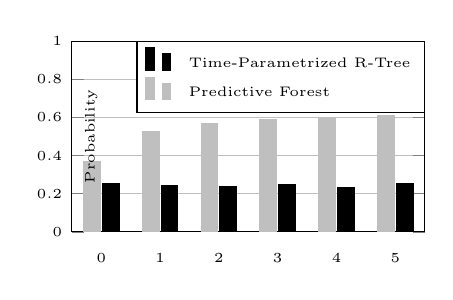
\begin{tikzpicture}
    \begin{axis}[
        width  = 0.5 * \textwidth,
        height = 4cm,
        major x tick style = transparent,
        ybar= 2 * \pgflinewidth,
        bar width=6pt,
        ymajorgrids = true,
        ylabel = {Probability},
        y label style={font=\tiny, at={(0.1,0.5)}},
        symbolic x coords={0, 1, 2, 3, 4, 5},
        x tick label style= {
                font=\tiny
            },
            y tick label style= {
                font=\tiny
            },
        xtick = data,
        scaled y ticks = false,
        enlarge x limits=0.1,
        ymin=0,
        ymax=1,
        legend cell align=left,
        every node near coord/.append style={font=\tiny},
        legend style={
                at={(1.0,1.0)},
                anchor=north east,
                column sep=1ex
        },
        reverse legend
    ]
        \addplot[style={lightgray,fill=lightgray,mark=none}]
            coordinates {
                (0, 0.3662)
                (1, 0.5267) % 0.6267
                (2, 0.5671) % 0.06471
                (3, 0.5889) % 0.6489
                (4, 0.6009) % 0.6489
                (5, 0.6100) % 0.6448
        };

        \addplot[style={black,fill=black,mark=none}]
             coordinates {
                (0, 0.2529)
                (1, 0.2412)
                (2, 0.2389)
                (3, 0.2494)
                (4, 0.2326)
                (5, 0.2545)
         };

        \legend{\tiny \PF, \tiny \TPR}
    \end{axis}
\end{tikzpicture}
\label{fig:accuracy0}
}
}}
\subfigure[Region radius 0.05 kilometer.]{
\vtop{\vskip0pt
\hbox{
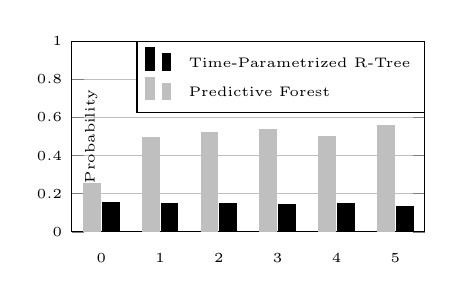
\begin{tikzpicture}
    \begin{axis}[
        width  = 0.5 * \textwidth,
        height = 4cm,
        major x tick style = transparent,
        ybar= 2 * \pgflinewidth,
        bar width=6pt,
        ymajorgrids = true,
        ylabel = {Probability},
        y label style={font=\tiny, at={(0.1,0.5)}},
        symbolic x coords={0, 1, 2, 3, 4, 5},
        x tick label style= {
                font=\tiny
            },
            y tick label style= {
                font=\tiny
            },
        xtick = data,
        scaled y ticks = false,
        enlarge x limits=0.1,
        ymin=0,
        ymax=1,
        legend cell align=left,
        every node near coord/.append style={font=\tiny},
        legend style={
                at={(1.0,1.0)},
                anchor=north east,
                column sep=1ex
        },
        reverse legend
    ]
        \addplot[style={lightgray,fill=lightgray,mark=none}]
            coordinates {
                (0, 0.2510)
                (1, 0.4924)
                (2, 0.5208)
                (3, 0.5383)
                (4, 0.4977)
                (5, 0.5568)
        };

        \addplot[style={black,fill=black,mark=none}]
             coordinates {
                (0, 0.1516)
                (1, 0.1501)
                (2, 0.1468)
                (3, 0.1448)
                (4, 0.1459)
                (5, 0.1335)
         };

        \legend{\tiny \PF, \tiny \TPR}
    \end{axis}
\end{tikzpicture}
\label{fig:accuracy05}}
}}
\subfigure[Region radius 0.1 kilometer.]{
\vtop{\vskip0pt
\hbox{
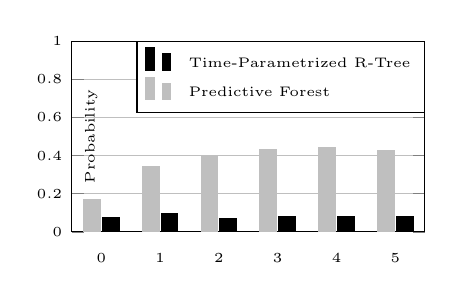
\begin{tikzpicture}
    \begin{axis}[
        width  = 0.5 * \textwidth,
        height = 4cm,
        major x tick style = transparent,
        ybar= 2 * \pgflinewidth,
        bar width=6pt,
        ymajorgrids = true,
        ylabel = {Probability},
        y label style={font=\tiny, at={(0.1,0.5)}},
        symbolic x coords={0, 1, 2, 3, 4, 5},
        x tick label style= {
                font=\tiny
            },
            y tick label style= {
                font=\tiny
            },
        xtick = data,
        scaled y ticks = false,
        enlarge x limits=0.1,
        ymin=0,
        ymax=1,
        legend cell align=left,
        every node near coord/.append style={font=\tiny},
        legend style={
                at={(1.0,1.0)},
                anchor=north east,
                column sep=1ex
        },
        reverse legend
    ]
        \addplot[style={lightgray,fill=lightgray,mark=none}]
            coordinates {
                (0, 0.1717)
                (1, 0.3444)
                (2, 0.4007)
                (3, 0.4339)
                (4, 0.4446)
                (5, 0.4275)
        };

        \addplot[style={black,fill=black,mark=none}]
             coordinates {
                (0, 0.0740)
                (1, 0.0951)
                (2, 0.0681)
                (3, 0.0806)
                (4, 0.0819)
                (5, 0.0801)
         };

        \legend{\tiny \PF, \tiny \TPR}
    \end{axis}
\end{tikzpicture}
\label{fig:accuracy1}
}
}}
\caption{Accuracy experiments for different region sizes}
\label{fig:accuracy}
\end{figure*}

\section{Scalability and Efficiency Evaluation}
The scalability experiments are applied to reveal how much \pf is scalable with respect of changing input parameters like radius size. In every experiment we scale one parameter and keep the others constants unchanged. The plots for the scalability experiments for CPU usage are in Figure ~\ref{fig:scalaCpu} and memory usage in Figure ~\ref{fig:scalaMem}

\begin{figure*}[ht]
\centering
\subfigure[Region Size.]{
\vtop{\vskip0pt
\hbox{
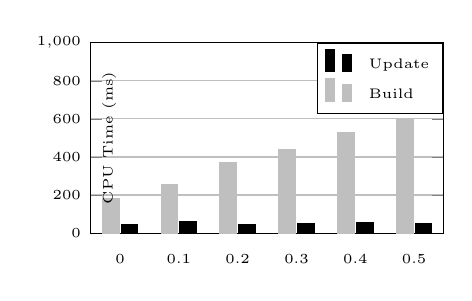
\begin{tikzpicture}
    \begin{axis}[
        width  = 0.5 * \textwidth,
        height = 4cm,
        major x tick style = transparent,
        ybar= 2 * \pgflinewidth,
        bar width=6pt,
        ymajorgrids = true,
        ylabel = {CPU Time (ms)},
        y label style={font=\tiny, at={(0.1,0.5)}},
        symbolic x coords={0, 0.1, 0.2, 0.3, 0.4, 0.5},
        x tick label style= {
                font=\tiny
            },
            y tick label style= {
                font=\tiny
            },
        xtick = data,
        scaled y ticks = false,
        enlarge x limits=0.1,
        ymin=0,
        ymax=1000,
        legend cell align=left,
        every node near coord/.append style={font=\tiny},
        legend style={
                at={(1.0,1.0)},
                anchor=north east,
                column sep=1ex
        },
        reverse legend
    ]
        \addplot[style={lightgray,fill=lightgray,mark=none}]
            coordinates {
                (0, 183.1303)
                (0.1, 253.7468) %753
                (0.2, 368.9956) % 1368
                (0.3, 436.7922) % 3236
                (0.4, 526.7508) % 4926
                (0.5, 602.3495) % 7402

        };
        \addplot[style={black,fill=black,mark=none}]
             coordinates {
                (0, 47.0653)
                (0.1, 63.0394)
                (0.2, 47.0371)
                (0.3, 52.1937)
                (0.4, 55.5097)
                (0.5, 52.0552)
         };

        \legend{\tiny Build, \tiny Update}
    \end{axis}
\end{tikzpicture}
\label{fig:scalaCpu0}
}}}
\caption{Scalability CPU Usage Experiments for \PF}
\label{fig:scalaCpu}
\end{figure*}

\begin{figure*}[ht]
\centering
\subfigure[Region Size.]{
\vtop{\vskip0pt
\hbox{
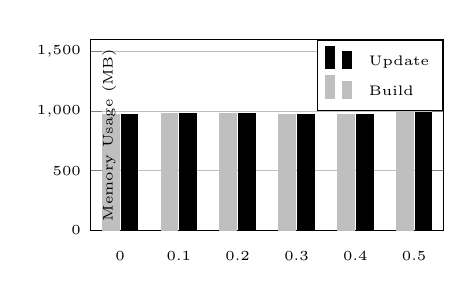
\begin{tikzpicture}
    \begin{axis}[
        width  = 0.5 * \textwidth,
        height = 4cm,
        major x tick style = transparent,
        ybar= 2 * \pgflinewidth,
        bar width=6pt,
        ymajorgrids = true,
        ylabel = {Memory Usage (MB)},
        y label style={font=\tiny, at={(0.1,0.5)}},
        symbolic x coords={0, 0.1, 0.2, 0.3, 0.4, 0.5},
        x tick label style= {
                font=\tiny
            },
            y tick label style= {
                font=\tiny
            },
        xtick = data,
        scaled y ticks = false,
        enlarge x limits=0.1,
        ymin=0,
        ymax=1600,
        legend cell align=left,
        every node near coord/.append style={font=\tiny},
        legend style={
                at={(1.0,1.0)},
                anchor=north east,
                column sep=1ex
        },
        reverse legend
    ]
        \addplot[style={lightgray,fill=lightgray,mark=none}]
            coordinates {
                (0, 973.8984375)
                (0.1, 976.46875)
                (0.2, 979.4140625)
                (0.3, 975.7109375)
                (0.4, 972.296875)
                (0.5, 991.19140625)

        };
        \addplot[style={black,fill=black,mark=none}]
             coordinates {
                (0, 973.8984375)
                (0.1, 976.46875)
                (0.2, 979.4140625)
                (0.3, 975.7109375)
                (0.4, 972.296875)
                (0.5, 991.19140625)
         };

        \legend{\tiny Build, \tiny Update}
    \end{axis}
\end{tikzpicture}
\label{fig:scalaMem0}
}}}
\caption{Scalability Memory Usage Experiments for \PF}
\label{fig:scalaMem}
\end{figure*}

\chapter{CONCLUSION}
\label{sect:conclusion}
In this paper we presented an incredible data structure for querying moving objects.

\bibliography{references}
\bibliographystyle{abbrv}

\end{document}
